\begin{frame}{Projekt przedwzmacniacza z modelem pseudo-rezystora w technologii $\SI{180}{\nano\metre}$  XFAB}
    \begin{figure}[H]
        \centering
        \includegraphics[scale=0.8]{ch3/pseudo-lay.pdf} 

    \end{figure}


\end{frame}

\begin{frame}{Wpływ pojemnościowych prądów bramki pseudo-rezystorów na zniekształcenia  w technologii $\SI{180}{\nano\metre}$}
    \vspace{-5mm} %5mm vertical space

    \begin{columns}
        \column{.3\textwidth}
        \begin{figure}[H]

            \includegraphics[trim={0 0.25cm 0 0.25cm}, clip, scale = 0.6]{scripts/tmp/IdsA.pdf}

        \end{figure}
        \column{.3\textwidth}
        \begin{figure}[H]

            \includegraphics[trim={0 0.25cm 0 0.25cm}, clip, scale = 0.6]{scripts/tmp/IdsB.pdf}

        \end{figure}
        \column{.3\textwidth}
        \begin{figure}[H]

            \includegraphics[trim={0 0.25cm 0 0.25cm}, clip, scale = 0.6]{scripts/tmp/IgbA.pdf}

        \end{figure}

    \end{columns}
    \vspace{-10mm} %5mm vertical space
    \begin{columns}
        \column{.3\textwidth}
        \begin{figure}[H]

            \includegraphics[trim={0 0.25cm 0 0.25cm}, clip, scale = 0.6]{scripts/tmp/IgbB.pdf}

        \end{figure}
        \column{.3\textwidth}
        \begin{figure}[H]

            \includegraphics[trim={0 0.25cm 0 0.25cm}, clip, scale = 0.6]{scripts/tmp/vOut.pdf}

        \end{figure}
        \column{.3\textwidth}
        \begin{figure}[H]

            \includegraphics[trim={0 0.25cm 0 0.25cm}, clip, scale = 0.6]{scripts/tmp/Igb_diff.pdf}

        \end{figure}

    \end{columns}
        



\end{frame}


\begin{frame}{Skalowanie zniekształceń z powierzchnią bramki i grubością tlenku tranzystorów tworzących pseudo-rezystory}
    \begin{columns}
        \column{.48\textwidth}
        \begin{block}{Powierzchnia bramki -- technologia $\SI{180}{\nano\metre}$ }
            \begin{figure}[H]
                \centering
                \includegraphics[scale = 0.7]{scripts/analyseTran/analyseTranSize.pdf}
            \end{figure}
        \end{block}

        \column{.48\textwidth}
        \begin{block}{Zależnosć od technologii}
            \begin{figure}[H]
                \centering
                \includegraphics[scale = 0.7]{scripts/analyseTran/analyseTranTechnology.pdf}
            \end{figure}
        \end{block}


    \end{columns}

\end{frame}

\begin{frame}{Szumy}
    \vspace{-5mm} %5mm vertical space

    \begin{columns}
    \column{.3\textwidth}
    \begin{figure}[H]
        \centering
        \includegraphics[scale=0.5]{ch2/conceptAC_Harrison.pdf} 
    \end{figure}
        \column{.3\textwidth}
        \begin{figure}[H]
            \centering
            \includegraphics[scale = 0.5]{scripts/tmp/fig3_R1.pdf}
        \end{figure}
        \column{.3\textwidth}
        \begin{figure}[H]
            \centering
            \includegraphics[scale = 0.5]{scripts/tmp/fig3_R2.pdf}
        \end{figure}
    \end{columns}

    \vspace{-5mm} %5mm vertical space


    \begin{columns}
        \column{.3\textwidth}
        \begin{figure}[H]
            \centering
            \includegraphics[scale=0.5]{scripts/noiseOutResistors/fig1_R1.pdf}
        \end{figure}
        \column{.3\textwidth}
        \begin{figure}[H]
            \centering
            \includegraphics[scale=0.5]{scripts/noiseOutResistors/fig2.pdf}
        \end{figure}
    \end{columns}


\end{frame}


\begin{frame}{Blok korekcji}
\begin{columns}

    \column{.35\textwidth}
    \begin{block}{
        Projekt kanału}
        \begin{figure}[H]
            \centering
            \includegraphics[scale = 0.4]{ch4/chap4Scheme.pdf}
        \end{figure} 
        \end{block}

        \begin{block}{
            Wyzwania do rozwiązania}
            \begin{figure}[H]
                \centering
                \includegraphics[scale = 0.6]{ch4/vgs_corr_sch.pdf} 
            \end{figure}   
            \end{block}



    \column{.6\textwidth}
    \begin{columns}
    \column{.45\textwidth}

    \begin{figure}[H]
        \centering
        \includegraphics[scale = 0.45]{scripts/tmp/analyseVgsTHD_1.pdf}
    \end{figure} 
    \column{.45\textwidth}
    \begin{figure}[H]
        \centering
        \includegraphics[scale =0.45]{scripts/tmp/analyseVgsTHD_2.pdf}
    \end{figure} 
    \end{columns}   

    \begin{columns}
    \column{.45\textwidth}

    \begin{figure}[H]
        \centering
        \includegraphics[scale = 0.4]{ch4/vgs_corr0.pdf}
    \end{figure} 
    \column{.45\textwidth}
    \begin{figure}[H]
        \centering
        \includegraphics[scale = 0.4]{ch4/vgs_corr1.pdf}
    \end{figure} 
    \end{columns}   
\end{columns}  
\end{frame}



\begin{frame}{Pomiary zniekształceń harmonicznych -- wpływ korekty}

    \begin{columns}

        \column{.45\textwidth}
        \begin{block}{Brak globalnej korekty}
            \begin{figure}[H]
                \centering
                \includegraphics[scale = 0.85]{scripts/tmp/thdFreqCorr0_0.pdf} 
            \end{figure}   
        \end{block}

        \column{.45\textwidth}

        \begin{block}{Korekta globalna}
            \begin{figure}[H]
                \centering
                \includegraphics[scale = 0.85]{scripts/tmp/thdFreqCorr100_0.pdf}
            \end{figure}   
        \end{block}
    \end{columns}

\end{frame}

\begin{frame}{Jednorodność kanałów}
    \begin{figure}[H]
        \centering
        \begin{subfigure}[b]{0.485\textwidth}
            \centering
            \includegraphics{scripts/tmp/bodePlotFc_0.pdf}

        \end{subfigure}
        % \hfill
        \begin{subfigure}[b]{0.485\textwidth}
            \centering
            \includegraphics{scripts/tmp/bodePlotFc_1.pdf}

        \end{subfigure}     
    \end{figure}
\end{frame}

\begin{frame}{Profil  lokalnego potencjału pola wywołanego (LFP) i rozkład  źródeł prądu (CSD)}
    \begin{figure}[H]


            \centering
            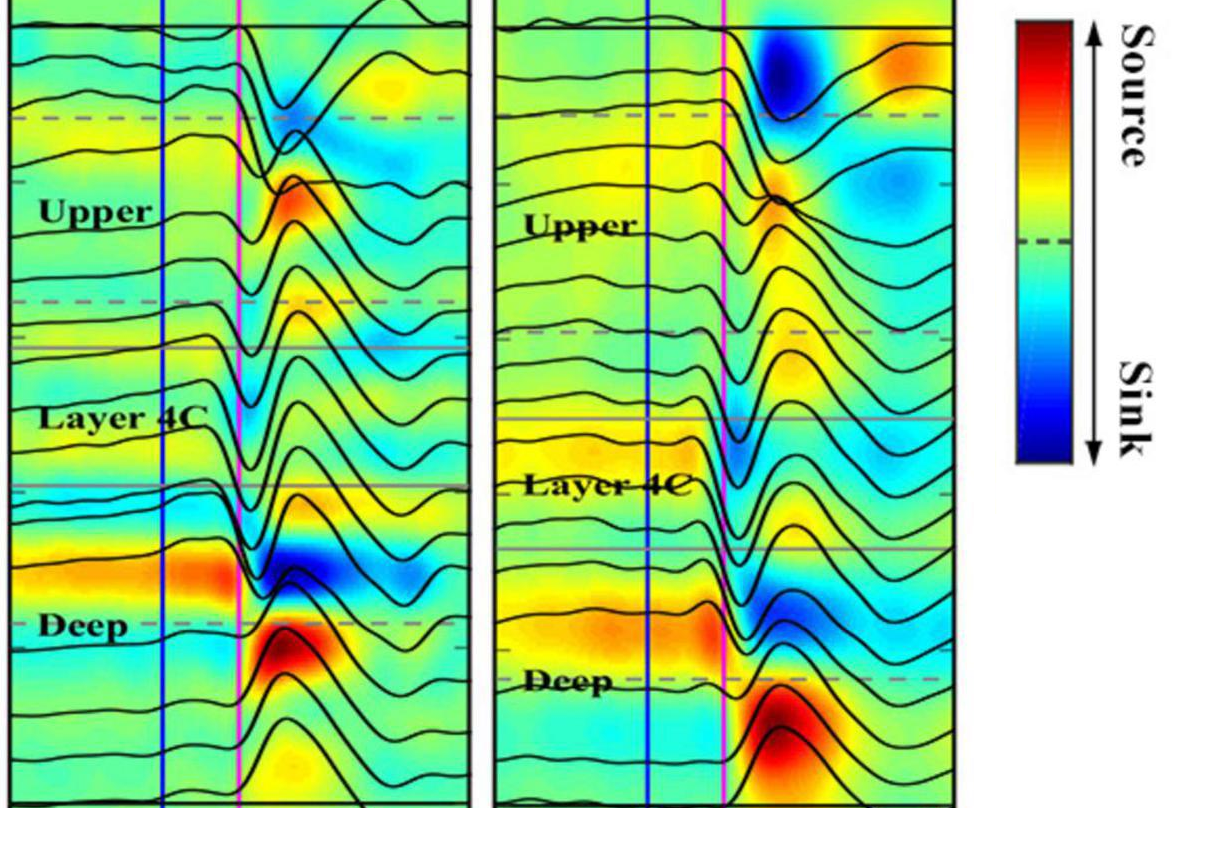
\includegraphics[scale=0.3]{Figures/lfp.png}

    
    \end{figure}
\end{frame}